\documentclass[11pt,oneside,final]{article}

\usepackage{mathtools}
\usepackage{accents}
\usepackage{amsmath}
\usepackage{amssymb}
\usepackage{amsthm}
\usepackage{centernot}
\usepackage{color}
\usepackage{enumerate}
\usepackage{geometry}
\usepackage{hyperref}
\usepackage{listings}
\usepackage{tabularx}
\usepackage{mathrsfs}
\usepackage{bbm}
\usepackage{subcaption}
\usepackage[table]{xcolor}
%PAGE FORMATTING
% \addtolength{\voffset}{-.4in}
% \addtolength{\hoffset}{0in}
% \addtolength{\footskip}{5pt}
% \addtolength{\textheight}{100pt}
\addtolength{\textwidth}{-20pt}
%% Shortcuts
\def\R{\mathbb R}
\def\RS{\mathbb S}
\def\Z{\mathbb Z}
\def\Q{\mathbb Q}
\def\C{\mathbb C}

%THEOREMS
\theoremstyle{definition}
\newtheorem{prb}{Problem}
\newtheorem*{prob}{\textbf{Problem :}}
\newtheorem*{prf}{Proof}
\newtheorem*{lem}{Lemma}
\newtheorem*{sln}{Solution}
\newtheorem*{fct}{Fact}
\newtheorem*{dfn}{Definition}
\newtheorem*{dfns}{Definitions}
\theoremstyle{theorem}
\newtheorem{cor}{Corollary}
\newtheorem{thm}{Theorem}
\newcommand{\irr}{\text{irr}}
\newcommand{\ol}[1]{\overline{#1}}
%NEW COMMANDS
\newcommand{\mc}[1]{\mathcal{#1}}
\newcommand{\bb}[1]{\mathbb{#1}}
\newcommand{\bbm}[1]{\mathbbm{#1}}
\newcommand{\ms}[1]{\mathscr{#1}}
\newcommand{\ttt}[1]{\texttt{#1}}
\newcommand{\includecode}[2][Python]{\lstinputlisting[caption=#2, escapechar=, style=custom#1]{#2}}
\newcommand{\embf}[1]{\textbf{\emph{#1}}}
\newcommand{\tbf}[1]{\textbf{#1}}
	% TOPOLOGY COMMANDS
\newcommand{\intr}[1]{\accentset{\circ}{#1}}
\newcommand{\bndr}{\partial}
\newcommand{\clsr}[1]{\overline{#1}}
\newcommand{\tpl}[1][]{\mathscr{T}_{#1}}
	% COMPLEX VARIABLE COMMANDS
\newcommand{\Log}{\text{Log}}
\newcommand{\partials}[2]{\frac{\partial #1}{\partial #2}}
\newcommand{\hessian}[3]{\left(\begin{array}{cc}\frac{\partial^2 #1}{\partial #2^2} & \frac{\partial^2 #1}{\partial #1 \partial #2} \\ \frac{\partial^2 u}{\partial #1\partial #2} & \frac{\partial^2 #1}{\partial #2^2}\end{array}\right)}
\newcommand{\Res}{\text{Res}}
%LISTING

\definecolor{mygreen}{rgb}{0,0.3,0.1}
\definecolor{mygray}{rgb}{0.5,0.5,0.5}
\definecolor{mymauve}{rgb}{0.58,0,0.82}
\definecolor{purple}{rgb}{0.78,0,0.82}
\definecolor{TEAL}{rgb}{0.2, 0.32, 0.5}
\definecolor{MAROON}{rgb}{0.55,0.051,0.12}
\definecolor{BEIGE}{rgb}{0.8,0.90,0.5}
\definecolor{AQUA}{rgb}{0.0, 0.8, 0.8}
\definecolor{GRAY90}{gray}{0.95}
\definecolor{GRAY80}{gray}{0.85}

\lstset{ %
  backgroundcolor=\color{white},   % choose the background color; you must add \usepackage{color} or \usepackage{xcolor}
  basicstyle=\footnotesize,        % the size of the fonts that are used for the code
  breakatwhitespace=false,         % sets if automatic breaks should only happen at whitespace
  breaklines=true,                 % sets automatic line breaking
  captionpos=b,                    % sets the caption-position to bottom
  commentstyle=\itshape\color{mygreen},
  deletekeywords={...},            % if you want to delete keywords from the given language
  escapeinside={\%*}{*)},          % if you want to add LaTeX within your code
  extendedchars=true,              % lets you use non-ASCII characters; for 8-bits encodings only, does not work with UTF-8
  frame=double,                    % adds a frame around the code
  keepspaces=true,                 % keeps spaces in text, useful for keeping indentation of code (possibly needs columns=flexible)
  keywordstyle=\bfseries\color{blue},       % keyword style
  language=Python,                 % the language of the code
  otherkeywords={*,...},            % if you want to add more keywords to the set
  numbers=left,                    % where to put the line-numbers; possible values are (none, left, right)
  numbersep=8pt,                   % how far the line-numbers are from the code
  numberstyle=\tiny\color{black}, % the style that is used for the line-numbers
  rulecolor=\color{black},         % if not set, the frame-color may be changed on line-breaks within not-black text (e.g. comments (green here))
  showspaces=false,                % show spaces everywhere adding particular underscores; it overrides 'showstringspaces'
  showstringspaces=false,          % underline spaces within strings only
  showtabs=false,                  % show tabs within strings adding particular underscores
  stepnumber=1,                    % the step between two line-numbers. If it's 1, each line will be numbered
  stringstyle=\color{mymauve},     % string literal style
  tabsize=2,                       % sets default tabsize to 4 spaces
  title=none                   % show the filename of files included with \lstinputlisting; also try caption instead of title
}

% LISTING STYLES
% customPython
\lstdefinestyle{customPython}{
  backgroundcolor=\color{BEIGE},
  belowcaptionskip=1\baselineskip,
  breaklines=true,
  frame=lines,
  numbers=left,
  xleftmargin=\parindent,
  language=Python,
  showstringspaces=false,
  basicstyle=\footnotesize\ttfamily,
  keywordstyle=\ttfamily\color{blue},
  commentstyle=\ttfamily\color{mygreen},
  identifierstyle=\color{TEAL},
  stringstyle=\color{MAROON},
  caption=
}
\lstdefinestyle{customPythonSnippit}{
  backgroundcolor=\color{BEIGE},
  belowcaptionskip=1\baselineskip,
  breaklines=true,
  frame=none,
  %xleftmargin=\parindent,
  language=Python,
  showstringspaces=false,
  basicstyle=\footnotesize\ttfamily,
  keywordstyle=\ttfamily\color{blue},
  commentstyle=\ttfamily\color{mygreen},
  identifierstyle=\color{TEAL},
  stringstyle=\color{MAROON},
  numbers=none,
  caption=
}
% customBash
\lstdefinestyle{customBash}{
  backgroundcolor=\color{BEIGE},
  belowcaptionskip=1\baselineskip,
  breaklines=true,
  frame=lines,
  xleftmargin=\parindent,
  language=Bash,
  showstringspaces=false,
  basicstyle=\footnotesize\ttfamily,
  keywordstyle=\ttfamily\color{blue},
  commentstyle=\ttfamily\color{mygreen},
  identifierstyle=\color{blue},
  stringstyle=\color{blue},
  caption=
}
% href setup
\hypersetup{pdfborder={0 0 0}, urlcolor=blue, linkcolor=blue, colorlinks=true}

\usepackage{graphicx}
\usepackage{wrapfig}
\usepackage[font={small,it}]{caption}
\graphicspath{{img/}}



\addtolength{\voffset}{-.5in}
\addtolength{\hoffset}{-.8in}
\addtolength{\footskip}{-10pt}
\addtolength{\textheight}{110pt}
\addtolength{\textwidth}{1.7in}

% href setup
\hypersetup{pdfborder={0 0 0}, urlcolor=blue, linkcolor=blue, colorlinks=true}
\begin{document}
\title{Fractal Geometry and Computer-Generated Art}
\author{Ben Kushigian}
\date{Date}
\maketitle
\tableofcontents



%%%%%%%%%%%%%%%%%%%%%%%%%%%%%%%%%%  Begin  %%%%%%%%%%%%%%%%%%%%%%%%%%%%%%%%%%%%




%%%%%%%%%%%%%%%%%%%%%%%%%%%%%%%%%  Abstract  %%%%%%%%%%%%%%%%%%%%%%%%%%%%%%%%%%

\section{Abstract}

In this project I will delve into fractal geometry, computer generated visual
art, and how the two tie together. I will draw from set theory, topology,
manifold theory, the theory of dynamics. 





%__*__*__*__*__*__*__*__*_  Section: Preliminaries  *__*__*__*__*__*__*__*__*__


\section{Preliminaries}
I lay out some fundamental concepts that we will build on. Some of this will get 
advanced so skim over material if it seems too dense.


    %%%%%%%%%%%%%  Subsection: Fractals - Some Definitions  %%%%%%%%%%%%%%%

\subsection{Fractals - Some Definitions and Notions}
The term `fractal' is most likely familiar to you though one runs the risk of
being imprecise with its use. We briefly state how we use the term.\\
\begin{dfn} A \textbf{fractal} is a natural phenomenon or a mathematical set
	that exhibits a repeating pattern that displays at every scale. If the 
	replication is exactly the same at every scale, it is called a self-similar
	pattern.
	\cite{wikipedia-fractals}\\

\end{dfn}

        %%%%%%%%%%%%%%%%%%  Figure: British Coast  %%%%%%%%%%%%%%%%%%%%

These are very general and somewhat wishy-washy definitions - not really
definitions at all. However they will suffice for our purposes as long as we
note a couple things. Firstly, in nature recursive patterns must bottom out, so
we use the phrase ``at all scales" very loosely. A classic example of the
fractal geometry being exhibited in nature is looking at a coastline. There is,
at any `reasonable' scale (read \emph{not too close} and \emph{not too far
away}), a boundary between a land mass and the water that surrounds it. When we
ask what the length of the coastline is we will get differing results,
depending on what are base unit of measurement is.\\


\begin{wrapfigure}{r}{0.35\textwidth}
	\centering
	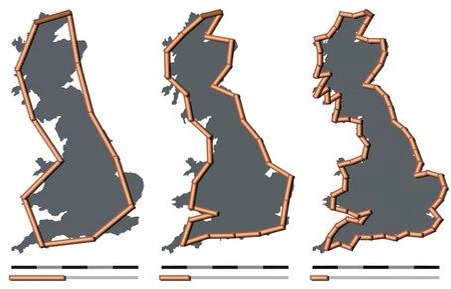
\includegraphics[width=0.34\textwidth]{Britain-fractal-coastline}
	\caption{The length of the coast of Britain with increasing precision -
	Taken from Wikipedia.com}
\end{wrapfigure}
In fact, coast lines exhibit a fractal nature. If you were given just the line
of the coast (say a part of the British coast, small enough to not have
distinctive features) and asked to guess what scale you were looking at it
would be impossible to tell. This is the essence of fractals. Note that there
is not `pattern' featured here, but rather the lack of a pattern. However we
may notice that the lack of a pattern is consistent - that is, the `roughness'
of the coastline is approximately the same at all scales. This brings us to
another definition of fractals which addresses this nuance.
\begin{dfn}
	A \textbf{fractal} is a curve or geometric figure, each part of which has
	the same statistical character as the whole.\cite{google}
\end{dfn}

Here we aren't talking about patterns anymore but statistical characteristics
of a set or curve. But this still doesn't quite get to the core of the matter.
We want to be able to cast aside degenerate examples such as lines or planes.
But the real line looks identical at all scales and fulfills both of our 
definitions so far.

\begin{thm}
	An open interval is homeomorphic to the real line.
\end{thm}
This is a topological theorem and we will later describe both what topology
is and what a homeomorphism is. For now it suffices to understand that in 
mathematics a morphism is a structure-preserving map from one object to another.
Morphisms are a way of formalizing similarities between different mathematical
structures.
\begin{proof}
	Let \(a < b\) be real numbers and so that the interval \((a,b)\) is well
	defined. We would like a bijective continuous open map \(\phi : (a,b)
	\rightarrow \mathbb R\). Without loss of generality assume that \(a =
	-\pi/2\) and \(b = \pi/2\) (a simple scale and translation allows us to do
	this and meets the requirements of \(\phi\)). Taking \(\phi(x) =
	\arctan(x)\) we have our desired result.
\end{proof}

This means that the real line is \emph{topologically identical} to an open
interval. A similar statement is true for an open disc in \(\mathbb R^2\) and
\(\mathbb R^2\) itself.  This brings us to our third and final definition of a
fractal:

\begin{dfn}
	\textbf{fractal}: You'll know it when you see it.
\end{dfn}

In truth we can supply more rigour by talking about \emph{fractional
dimensions}, and we will, though perhaps not at a great enough depth to
classify exactly {\em why} an open interval is not fractal.


        %%%%%%%%%%%%%  SubSection: Types Of Fractals  %%%%%%%%%%%%%%
\subsection{Types of Fractals}
There are many types of fractals and to my knowledge their categorizion is not
standardized. We enumerate a few of them here.\\



\begin{wrapfigure}{r}{0.35\textwidth}
	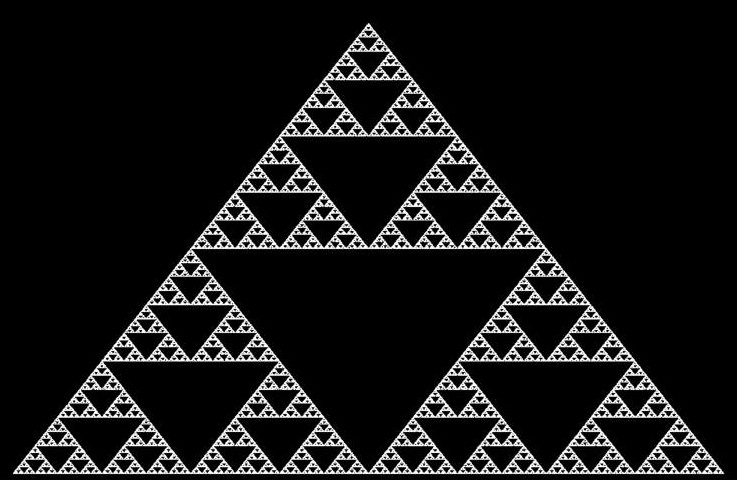
\includegraphics[width=0.35\textwidth]{sierpinski_32000-1}
	\caption{The Sierpinski Gaskett is a classic example of an IFS. Rendered in
	C++ using OpenGL}
\end{wrapfigure}

\noindent\textbf{Deterministic Iterated Funcion Systems (IFS)} This is a method
of constructing fractals that involves taking the union of several images of an
initial figure under \emph{contractive} \footnote{A contractive map \(f: U
\rightarrow V\) is a map with the property that for any two points in its
domain \(x\) and \(y\), \(|f(x) - f(y)| < |x-y|\).} maps \(f_1, f_2,
\ldots, f_n\) and repeating the process \emph{ad infinitum}.  Often these
maps are required to be linear or affine though many IFS fractals are
created with nonlinear functions. The classic example is the Sierpinski
Gaskett.  This mathematical oddity has many interesting properties, some of
which we will have a chance to look at. The basic affine transformation is
to make three copies of the original image contracted to half their
original size and place them in a triangular formation. \\

\begin{wrapfigure}{l}{0.35\textwidth}
	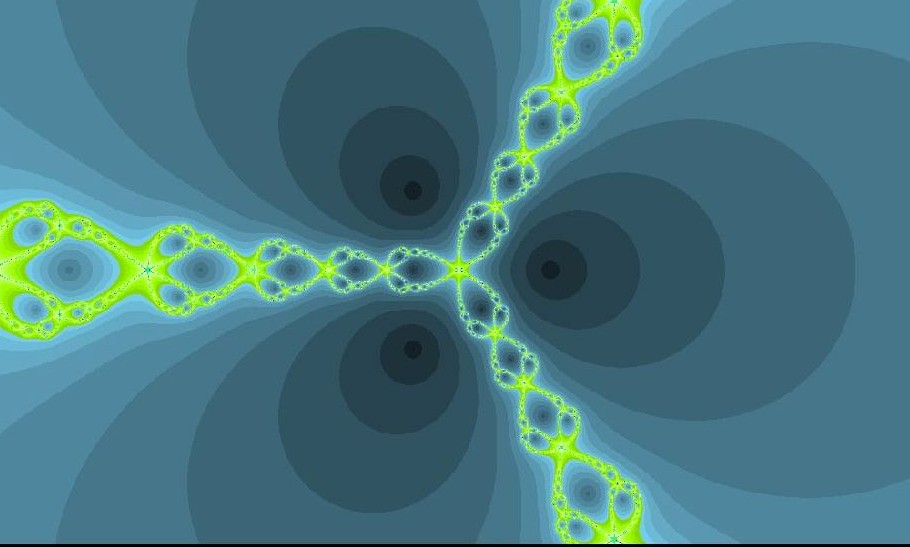
\includegraphics[width=0.35\textwidth]{newton_z3-1}
	\caption{The newton fractal for \(f(z) = z^3\). Rendered in C++ using OpenGL.}
\end{wrapfigure}

\begin{wrapfigure}{r}{0.25\textwidth}
	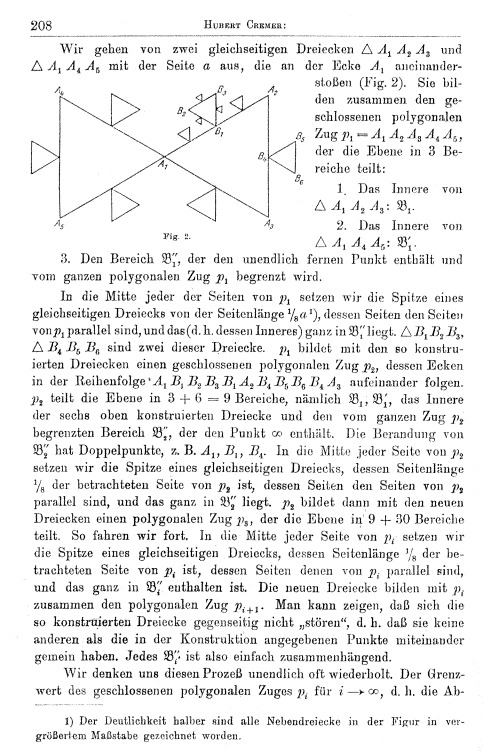
\includegraphics[width=0.25\textwidth]{julia_triangles}
	\caption{The Julia Set before computer graphics, drawn in 1924 by Hubert
	Cremer \cite{wahl}}
\end{wrapfigure}

\noindent\textbf{Complex-Dynamic Fractals (CDF)}
\begin{enumerate}[i]
	\item {\bf Newton Fractals:} Newton fractals use Newton's method of
		approximation in the complex plane to observe how a function tends to
		its roots.  While in the real case it is rather easy to predict where
		point will end up, in the complex case it is much more difficult.  
	\item {\bf Julia Sets:} The Julia set, named after mathematician Gaston
		Julia, is another fractal generated in the complex plane. From a very
		simple equation and endless iteration we get a glimpse at how dynamic
		the complex plane really is.
\end{enumerate}
\noindent\textbf{Physical Simulations} We have recently begun to notice the
order inherant in chaos - that behind much of the worlds seeming randomness
there is actually a very fine order; a beauty behind the clutter. Perhaps
one of the most striking visualizations of this is the {\em (Magnetic) Chaos 
Pendulum}. Here is the basic setup: We have a table on which lie three
magnets of equal charge and polarity, all equadistant from some center point
\(p\) and equadistant frome one another; that is they lie on a circle with
center \(p\) and describe an equilateral triangle.\\
Now associate with each magnet a color: Red, Yellow and Blue. We conduct
an experiment where we hang a magnetic pendulum above the table so that it
hangs down above the point \(p\). Assume that the pendulum is attracted to
each of the magnets, and assume that the attraction is powerful enough that 
the pendulum can be `affixed' at an angle so that it is held steady by one
of the magnets.\\
We take a birds eye view and let the pendulum be moved to occupy a point above
the table. We then release it and see, after a while, which magnet the pendulum
eventually ends up at. We color the point over which the pendulum initially hung
the color associated with the magnet. The image on your left is the result.

\begin{wrapfigure}{l}{0.25\textwidth}
	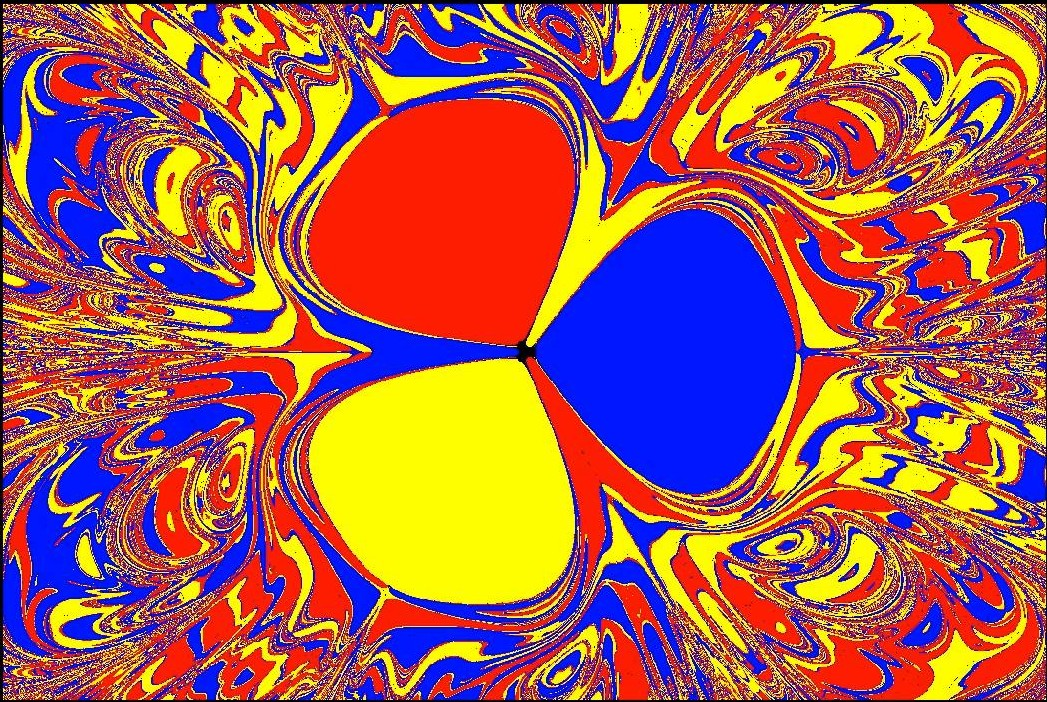
\includegraphics[width=0.25\textwidth]{chaos_pendulum1}
	\caption{The magnetic chaos pendulum, rendered in C++ using OpenGL.}
\end{wrapfigure}

        %%%%%%%%%%%%  SubSection: Fractals In Nature  %%%%%%%%%%%%%%
\subsection{Fractals in Nature}

    %%%%%%%%%%%%%%%%%%%  Subsection: Complex Numbers  %%%%%%%%%%%%%%%%%%%%%

\subsection{Complex Numbers} We assume some familiarity with complex numbers. We 
briefly state some facts that will be useful. First we talk about the 
\emph{\textbf{field} of complex numbers} and denote it \(\mathbb C\). We will 
also refer to complex numbers as existing in the \textbf{complex plane}. This
gives us a geometric handle on how these objects act.\\


        %%%%%%%%%%%%%%%%%%  Figure: Complex Plane  %%%%%%%%%%%%%%%%%%%%

\begin{wrapfigure}{l}{0.35\textwidth}
	\centering
	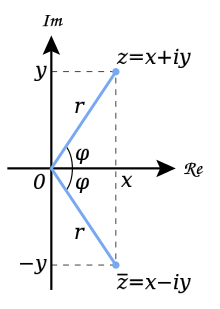
\includegraphics[width=0.35\textwidth]{complex_conj}
	\caption{Complex conjugate of \(z = x + iy\) with exponential form. Taken
	from Wikipedia.com}
\end{wrapfigure}
We denote complex numbers in a few ways. First we write them as ordered pairs
\(z = (x, y)\) where \(x\) is called the \emph{real part} and \(y\) is called 
the \emph{imaginary part}. This notation lets us work with \(\mathbb C\) as the
real plane \(\mathbb R^2\) with some extra structure (the multiplication
operation). We may also write \(z = (x,y) = x + iy\) where \(i\) represents
the square root of negative one: \(i = \sqrt{-1}\). Note that there are 
actually two square roots of negative one: \(i^2 = (-i)^2 = -1\). Finally it is
often convenient to write elements of \(\mathbb C^* = \mathbb C \setminus 
(0,0)\) in polar form: \(z = x + iy = r(\cos \theta + i\sin \theta)\), where
\(r = \sqrt{x^2 + y^2}\) and \(\theta\) is the angle of elevation from the 
positive real line (up to an additive term of \(2\pi i\)). By Euler's formula
we can write this as \(re^{i\theta}\). This is called the exponential form. Note
that exponential and polar form are not bijective.\\

We define addition in the same manner as addition in \(\mathbb R^2\):
\((x_1, y_1) + (x_2, y_2) = (x_1 + x_2, y_1 + y_2)\). Let \(w = x_1 + iy_1\)
and \(z = x_2 + iy_2\). We define multiplication \(w\cdot z\) as
\[w \cdot z = (x_1,y_1)(x_2,y_2) = (x_1 x_2 - y_1 y_2,\ x_1y_2 + x_2y_1).\]
Letting \(re^{i\theta} = z,\ se^{i\phi} = w\) be the exponential forms of 
\(z,w\) we can write \(zw = rse^{i(\phi + \theta)}\) and we see that complex
multiplication is a rotation composed with a dilation.

As stated, \(\mathbb C\) is a field under addition and operation, which means
\begin{enumerate}
	\item \(\mathbb C\) is an abelian group under addition;
	\item \(\mathbb C\setminus \{0\}\) is an abelian group under multiplication.  
\end{enumerate}
Both of these properties are easy to check. Further we note that \(\mathbb C\)
is the \textbf{extension field} of \(\mathbb R\) - that is, an \(n\)-degree
polynomial \(P[X]\) over \(\mathbb R\) has exactly \(n\) solutions counting
multiplicity in \(\mathbb C\), and \(\mathbb C\) has no proper subset with
this property (Fundamental Theorem of Algebra). \\

It will at times be useful to view \(\mathbb C\) as a subset of \(\mathbb S\),
the Riemann Sphere. We can imagine attaching a point at infinity, written
\(\mathbb S = \mathbb C \cup \{\infty\}\). This has the very nice property
that \(\mathbb S\) contains all of its limit points. We say it is
\textbf{limit-point compact} or simply \textbf{compact}. Compactness is a 
topological notion and in general compactness is stronger than limit-point
compactness. However in the Euclidean plane this the two are equivalent and we
lose no rigor switching between the terms.\\
Since \(\mathbb S\) is compact we call \(\mathbb S\) the \textbf{one-point
compactification of \(\mathbb C\)}. Compact topological spaces have many nice
features. Our main focus for considering \(\mathbb S\) instead of \(\mathbb C\)
is that we can consider functions such as \(\frac{1}{z}\) as a map from 
\(\mathbb S\) to \(\mathbb S\) if we define \(\frac{1}{0} = \infty\) and 
\(\frac{1}{\infty} = 0\). Additionally we will be discussing fractal basins,
attractors in \(\mathbb C\) for iterated functions. By dealing with
\(\mathbb S\) instead of \(\mathbb C\) this will unify our theory and simplify
concepts.




        %%%%%%%%%%%%  Subsection: Topology and Manifolds  %%%%%%%%%%%%%

\subsection{Topology and Manifolds} We will use some notions from topology
and manifold theory. First we define an open disc \(D(z_0, r)\) to be the
set of points \(\{z \in \mathbb C\ |\ |z - z_0| < r\}\). This is the familiar
definition. Then an \textbf{open set} in the complex plane is a set that can
be formed as
\[U = \bigcup_{\alpha\in J}D_\alpha,\]
where \(J\) is an arbitrary index set and \(D_\alpha\) is an open disc. The 
collection \(\{D(z_0, r)\ |\ z_0 \in \mathbb C,\, r \in \mathbb R^+\}\) is
called the \textbf{basis that generates \(\mathbb C\)}. \\

An \(n\)-manifold is a topological space that is locally euclidean, Hausdorff
and second-countable. We inspect these ideas briefly.


\begin{dfn} Let \(X,\ Y\) be topological spaces. We say that \(f: X \rightarrow
	Y\) is \textbf{continuous} if for every \(V \subset Y\) the pre-image \(U =
	f^{-1}(V) \subset X\) is open. We say that \(f\) is an \textbf{open map} if
	for every open set \(U \subset X\) the image \(f(U)\) is open in \(Y\). We 
	say that the map \(f\) is \textbf{bijective} if it is onto and into.
	Finally we say that \(f\) is a \textbf{homeomorphism} if it is a continuous 
	open bijection. If \(f: X \rightarrow Y\) is a homeomorphic then we say 
	that \(X\) is homeomorphic to \(Y\) and write \(X \approxeq Y\). 
\end{dfn}
We leave the following statement unproved (it is a simple exercise if the
reader is interested).
\begin{thm} Homeomorphism is an equivalence relation. \end{thm}

We define three terms needed to define a manifold.
\begin{dfn} A space \(X\) is \textbf{locally Euclidean} 
if for every point \(x \in X\) we may find an open set \(U \subset X\) with 
a homeomorphism \(\phi: U \rightarrow \tilde{U} \subset \mathbb R^n\).
\end{dfn}

\begin{dfn} A space \(X\) is \textbf{Hausd\"orff} if for every pair of distinct
points \(x,y \in X\) we may find open sets \(U, V \subset X\) so that \(x \in
U, y \in V,\ U\cap V = \varnothing\).  

\end{dfn}

\begin{dfn} A space \(X\) is \textbf{Second Countable} if it has a countable
	basis. 
\end{dfn}

The most 


%%%%%%%%%%%%%%%%%%%%%%%%%%%%%%%%% Bibliography %%%%%%%%%%%%%%%%%%%%%%%%%%%%%%%%%%
\addcontentsline{toc}{section}{References}
\begin{thebibliography}{9}
\bibitem{fractalfoundation}
	\textit{The Fractal Foundation}
	\\\texttt{http://fractalfoundation.org/}
\bibitem{chaosandfractals}
	Peitgen, J\"urgens and Saup
	\textit{Chaos and Fractals}
	Springer-Verlag, New York, New York, 1992.
\bibitem{google}
	\textit{Google Search}
	\\\texttt{https://www.google.com}
\bibitem{wikipedia-fractals}
	\textit{Wikipedia - Fractals}
	\\\texttt{https://en.wikipedia.org/wiki/Fractal}
\bibitem{wahl}
	\textit{wahl.org}
	\\\textit{http://benkushigian.com/misc/pdfs/defs455.pdf}
\end{thebibliography}
\end{document}
